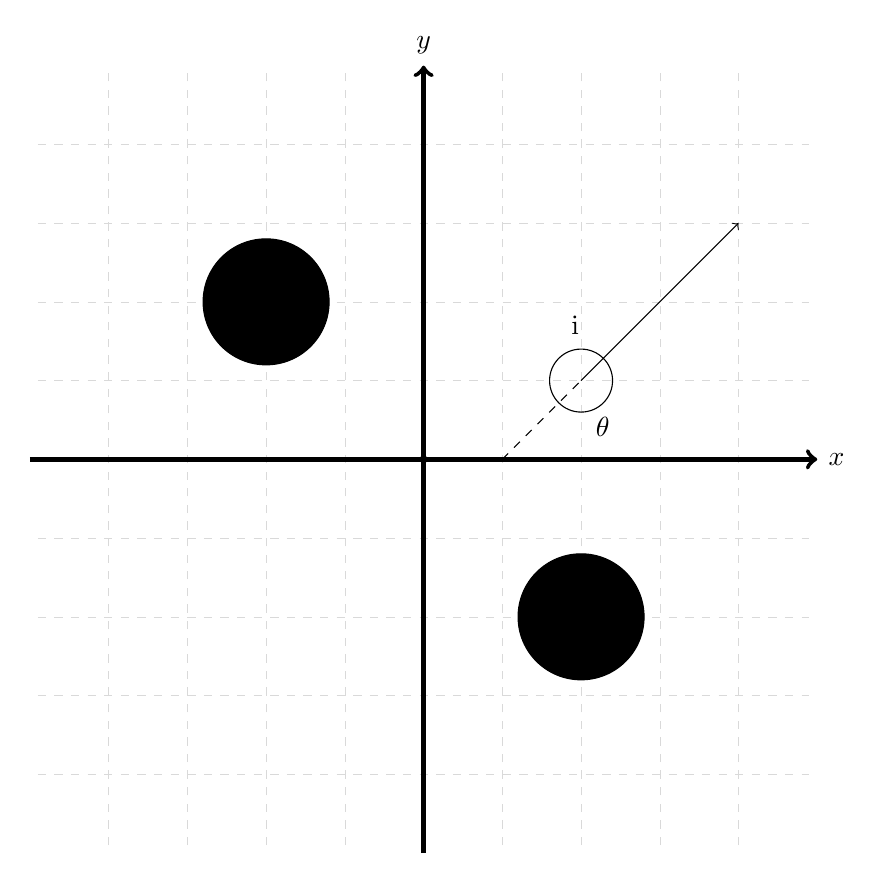
\begin{tikzpicture}
\draw[help lines, color=gray!30, dashed] (-4.9,-4.9) grid (4.9,4.9);
\coordinate (origo) at (0,0);
\coordinate (origo1) at (1.45,0);
\fill[black] (origo) circle (0.05);
\draw[->,ultra thick] (-5,0)--(5,0) node (x) [right]{$x$};
\draw[->,ultra thick] (0,-5)--(0,5) node (y) [above]{$y$};
\draw[] (2.1,1.7) node (i) [left]{i};
\draw[dashed] (1,0)--(2,1);
\draw[->] (2,1)--(4,3);
\draw (x) +(172:3) node {$\theta$};
\tkzDrawArc[R with nodes,](origo1,0.4)(x,y)


\draw[fill] (-2,2) circle [radius=0.8];
\draw[fill] (2,-2) circle [radius=0.8];
\draw (2,1) circle [radius=0.4];
\end{tikzpicture}
